\documentclass[12pt]{article}
\usepackage[italian]{babel} % imposta lingua
\usepackage[babel]{csquotes} % imposta lingua
\usepackage[utf8]{inputenc} % imposta lingua
\usepackage[T1]{fontenc} % imposta lingua
\usepackage{amsmath, amssymb, amsfonts} % pachetto per formule
% \usepackage[parfill]{parskip} % non si dovrebbe fare, ma sostituisce le rientranze dei paragrafi con interlinea
\usepackage{listings} % per poter far riconoscere e colorare codice 
\usepackage{xcolor} % pacchetto per testo colorato
\usepackage{float, subfig} % pachetto per figure, per posizionamento
\usepackage{booktabs} % pacchetto per tabelle
\usepackage{graphicx, wrapfig} % pachetto per tabelle
\usepackage{tcolorbox} % riquadri colorati
\usepackage[Listato]{algorithm} % pseudocodice
\usepackage{algpseudocode} % pseudocodice
\usepackage[hidelinks]{hyperref} % indice e riferimenti cliccabili e senza riquadro rosso
\frenchspacing %spaziatura italiana per accenti
\usepackage[colorinlistoftodos,prependcaption,textsize=tiny]{todonotes} % note TODO
% CONFIGURAZIONE LINK E RIFERIMENTI
\hypersetup{%
	pdfpagemode={UseOutlines},
	bookmarksopen,
	pdfstartview={FitH},
	colorlinks,
	linkcolor={black}, %COLORE DEI RIFERIMENTI AL TESTO
	citecolor={blue}, %COLORE DEI RIFERIMENTI ALLE CITAZIONI
	urlcolor={blue} %COLORI DEGLI URL
}

\begin{document}

\begin{titlepage}

\newcommand{\HRule}{\rule{\linewidth}{0.5mm}} % Defines a new command for the horizontal lines, change thickness here

\center % Center everything on the page
 
%----------------------------------------------------------------------------------------
%	HEADING SECTIONS
%----------------------------------------------------------------------------------------

\textsc{\LARGE Università degli studi di Milano-Bicocca}\\[1cm] % Name of your university/college
\textsc{\Large Advanced Machine Learning }\\[0.3cm] % Major heading such as course name

%----------------------------------------------------------------------------------------
%	TITLE SECTION
%----------------------------------------------------------------------------------------

\HRule \\[0.4cm]
{ \huge \bfseries Tox21 Grand Challenge}\\[0.4cm] % Title of your document
\HRule \\[1.5cm]
 
%----------------------------------------------------------------------------------------
%	AUTHOR SECTION
%----------------------------------------------------------------------------------------

\large
Mistri Matteo - 808097 \\   % Your name
Papetti Daniele Maria - 808027 \\[1cm] % Your name

% If you don't want a supervisor, uncomment the two lines below and remove the section above
%\Large \emph{Author:}\\
%John \textsc{Smith}\\[3cm] % Your name

%----------------------------------------------------------------------------------------
%	DATE SECTION
%----------------------------------------------------------------------------------------

{\large \today}\\[2cm] % Date, change the \today to a set date if you want to be precise

%----------------------------------------------------------------------------------------
%	LOGO SECTION
%----------------------------------------------------------------------------------------


\includegraphics{../images/pdf/logo}\\[1cm] % Include a department/university logo - this will require the graphicx package
 
%----------------------------------------------------------------------------------------

\vfill % Fill the rest of the page with whitespace

\end{titlepage}

\pagenumbering{arabic}
\begin{abstract}
Lo scopo di questo lavoro è quello di sviluppare una rete neurale per la classificazione di composti chimici in base alla possibile tossicità rispetto ad alcuni \textit{pathways} cellulari; il dataset utilizzato per la prova è \href{http://bioinf.jku.at/research/DeepTox/tox21.html}{Tox21}.
In primo luogo, è stata evidenziata la natura multi-label del problema (\textit{i.e.}, 12 label differenti di cui predire il valore); inoltre, è stato mostrato come il dataset sia estremamente sbilanciato per ogni label, evidenziando l'impossibilità di bilanciarlo a causa della natura delle etichette.
Dopo aver effettuato operazioni di \textit{preprocessing}, è stato brevemente indagato come la profondità della rete neurale influisse sulle performance del modello; i risultati mostrano come una profondità maggiore non garantisca prestazioni migliori, portando a scegliere per il lavoro un rete con tre layer nascosti.
Successivamente è stato effettuato un processo di ottimizzazione degli iperparametri, al fine di individuarne la configurazione ottima e stabilire quale tra quattro possibili input preprocessati della rete utilizzare.
Infine è stato addestrato il modello con la configurazione di iperparametri e input ottimale, confrontandone le performance con altri modelli presenti in letteratura.
I risultati mostrano che l'approccio proposto si posiziona a “metà classifica”, con performance parzialmente peggiori rispetto a varie tecniche \textit{ensamble}.
\end{abstract}

\section{Introduzione}
Il problema affrontato in questo lavoro è quello dello sviluppo di un classificatore per i dataset Tox21 \cite{challenge_site}, una \textit{challenge} proposta dal \textit{U.S. Department of Health and Human Services} che consiste nel predire il risultato di dodici differenti test tossicologici eseguiti su delle molecole a partire da un insieme di descrittori della struttura chimica dei composti proposti.
L'obiettivo della cosiddetta \textit{Grand Challenge}, affrontata in questo lavoro, è quello di predire il risultato di tutti e dodici le etichette contemporaneamente. I test possono essere catalogati in due macro-gruppi: i primi $7$, identificati dal prefisso \textit{NR}, afferiscono all'area dei test relativi ai \textit{pathways} di segnalazione dei recettori nucleari (\textit{nuclear receptor effects}); i restanti $5$, identificati dal prefisso \textit{SR}, sono relativi alla risposta cellulare agli stress (\textit{stress responde effects}).
Analizzando i dati, si evince che il problema risulta essere fortemente sbilanciato e senza possibilità di bilanciamento, vista la natura multi-label della predizione.
Per l'individuazione di un classificatore ottimale al fine di svolgere la \textit{challenge}, sono stati posti i seguenti obiettivi: (i) confrontare diverse topologie di rete; (ii) individuare la tecnica di feature reduction ottimale; (iii) determinare tramite un processo di ottimizzazione la configurazione migliore di iperparametri per i modelli ; (iv) analizzare le performance del modello individuato.

\section{Dataset utilizzato}
Il dataset utilizzato per il progetto è stato prelevato dal sito \cite{dataset_site}, che mette a disposizione i dati di train ($12060$ \textit{sample}) e di test ($647$ \textit{sample}) per lo svolgimento della \textit{challenge} associata al problema.
Ogni elemento del dataset rappresenta un differente composto chimico ed è caratterizzato da un insieme di $801$ feature dense e oltre $200000$ feature sparse. Considerata la complessità computazionale aggiuntiva derivante dall'utilizzo di queste ultime feature a fronte della minima quantità di informazione apportata, è stato deciso di non considerare la porzione sparsa della matrice, come consigliato dal sito citato in precedenza.
Ad ogni \textit{sample} è associato un vettore binario di etichette contenente $12$ elementi.
Ognuno di essi corrisponde al risultato di una differente analisi tossicologica a cui la molecola è stata sottoposta. Le analisi effettuate possono essere unite in due macro-gruppi: le prime $7$, identificate dal prefisso NR (\textit{nuclear receptor effects}), afferiscono all'area dei test relativi ai \textit{pathways} di segnalazione dei recettori nucleari; le restanti $5$, identificate dal prefisso SR (\textit{stress responde effects}), sono relative alla risposta cellulare agli stress.

L'analisi della matrice delle etichette ha mostrato una discreta presenza di valori \texttt{NaN} (35\% nel train set, 10\% nel test set); non essendo presente alcuna motivazione di questi valori nella descrizione del dataset, è stato supposto che alcune analisi siano state tralasciate per quelle molecole che i ricercatore hanno ritenuto certamente non tossiche in determinati \textit{pathways}. Per questo motivo, tutti i valori \texttt{NaN} sono stati sostituiti con $0$, rappresentando quindi un esito del test tossicologico negativo per il composto chimico.\\
\begin{figure}[!ht]
	\centering
	\subfloat{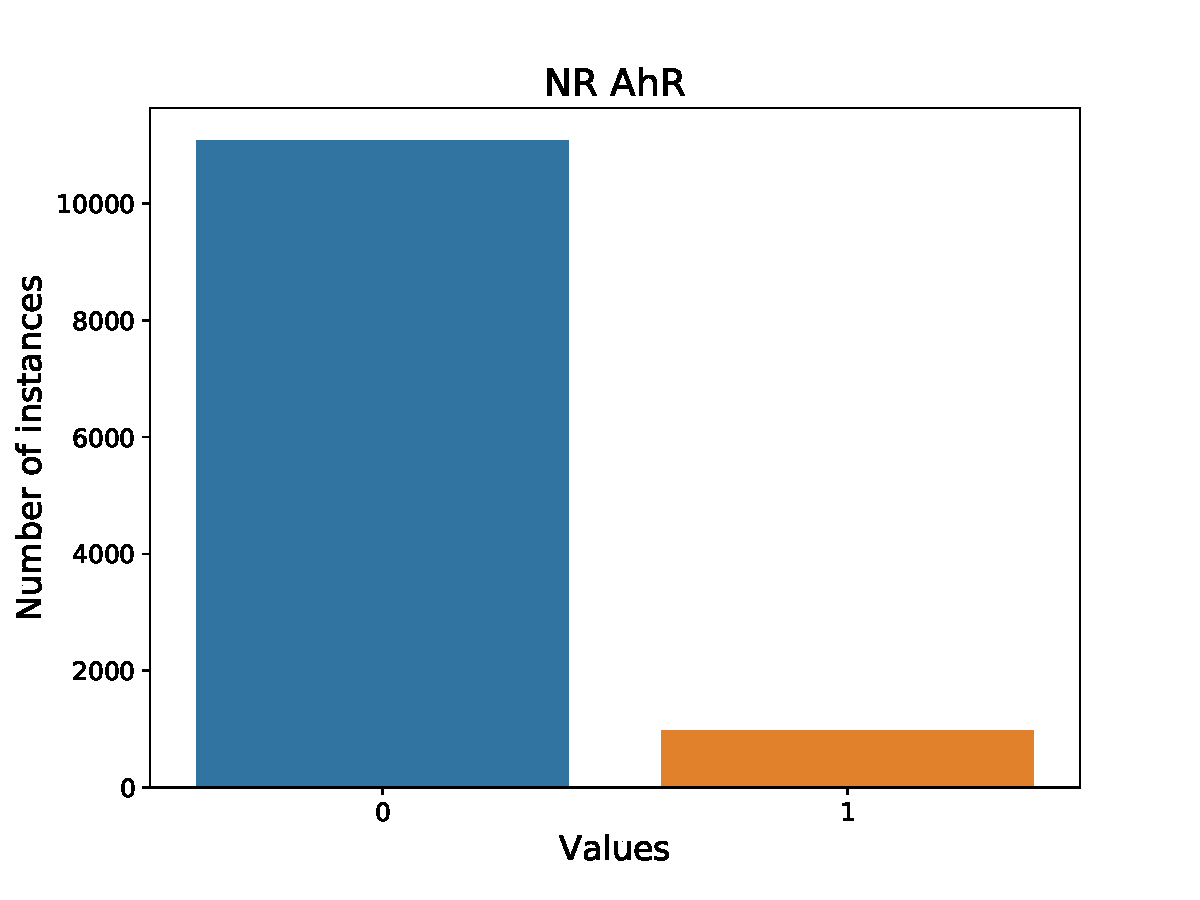
\includegraphics[width=.2\textwidth]{../images/pdf/hist-NRAhR}}\quad
	\subfloat{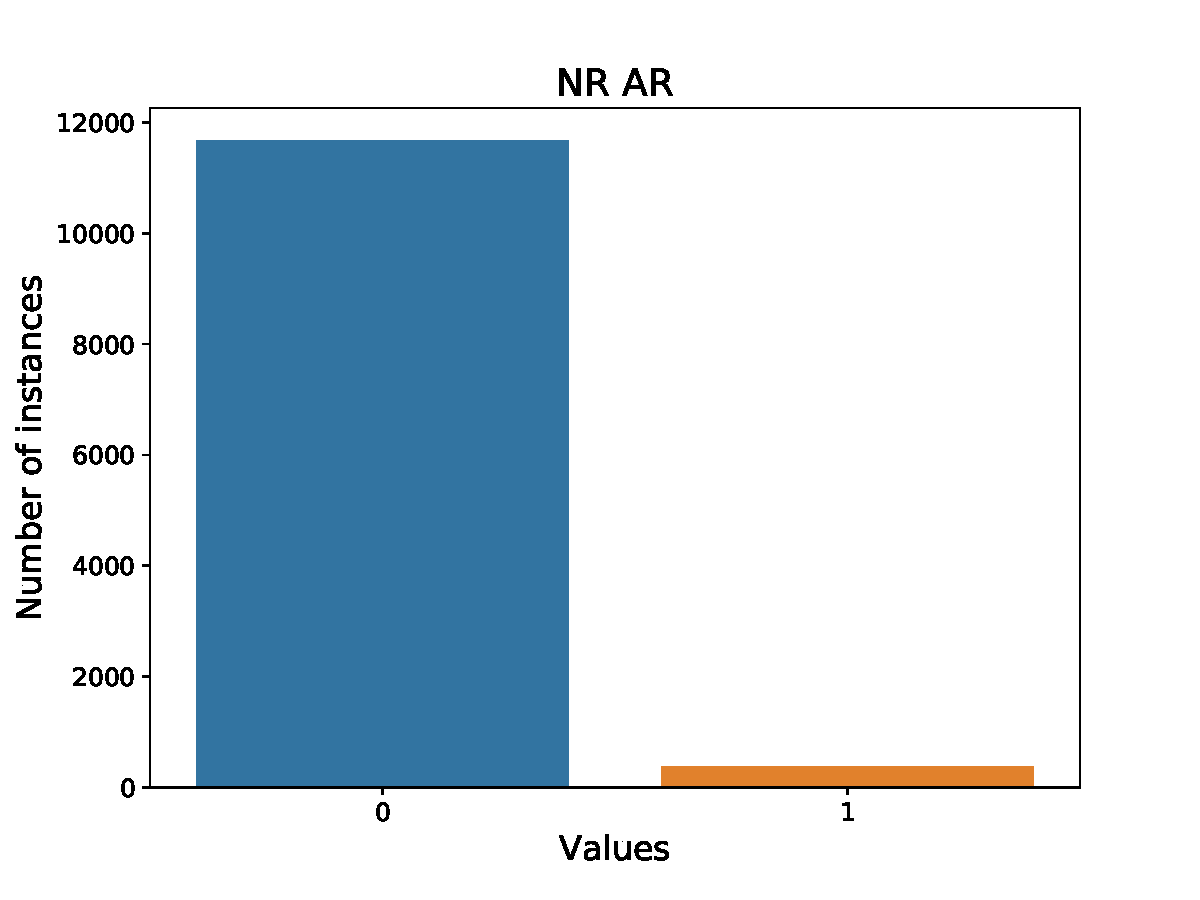
\includegraphics[width=.2\textwidth]{../images/pdf/hist-NRAR}}\quad
	\subfloat{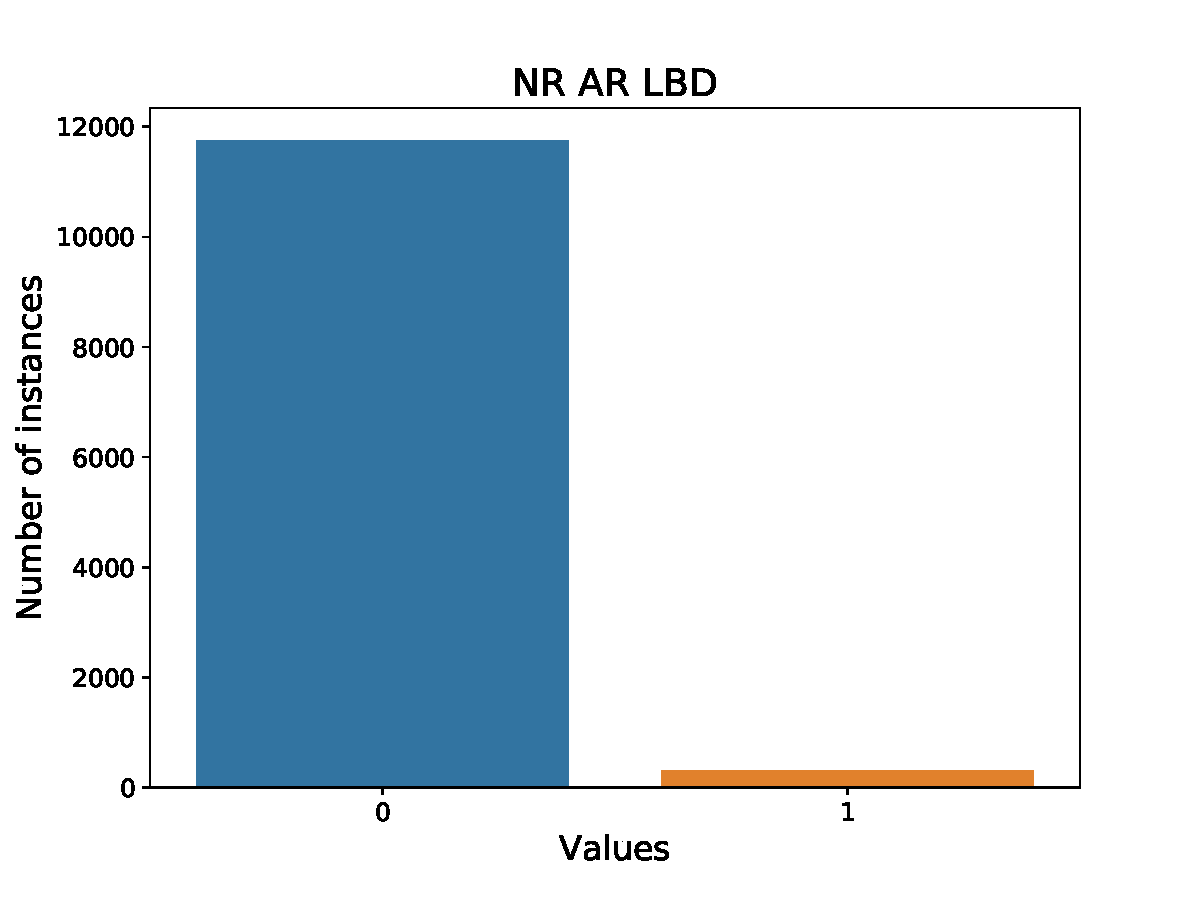
\includegraphics[width=.2\textwidth]{../images/pdf/hist-NRARLBD}}\quad
	\subfloat{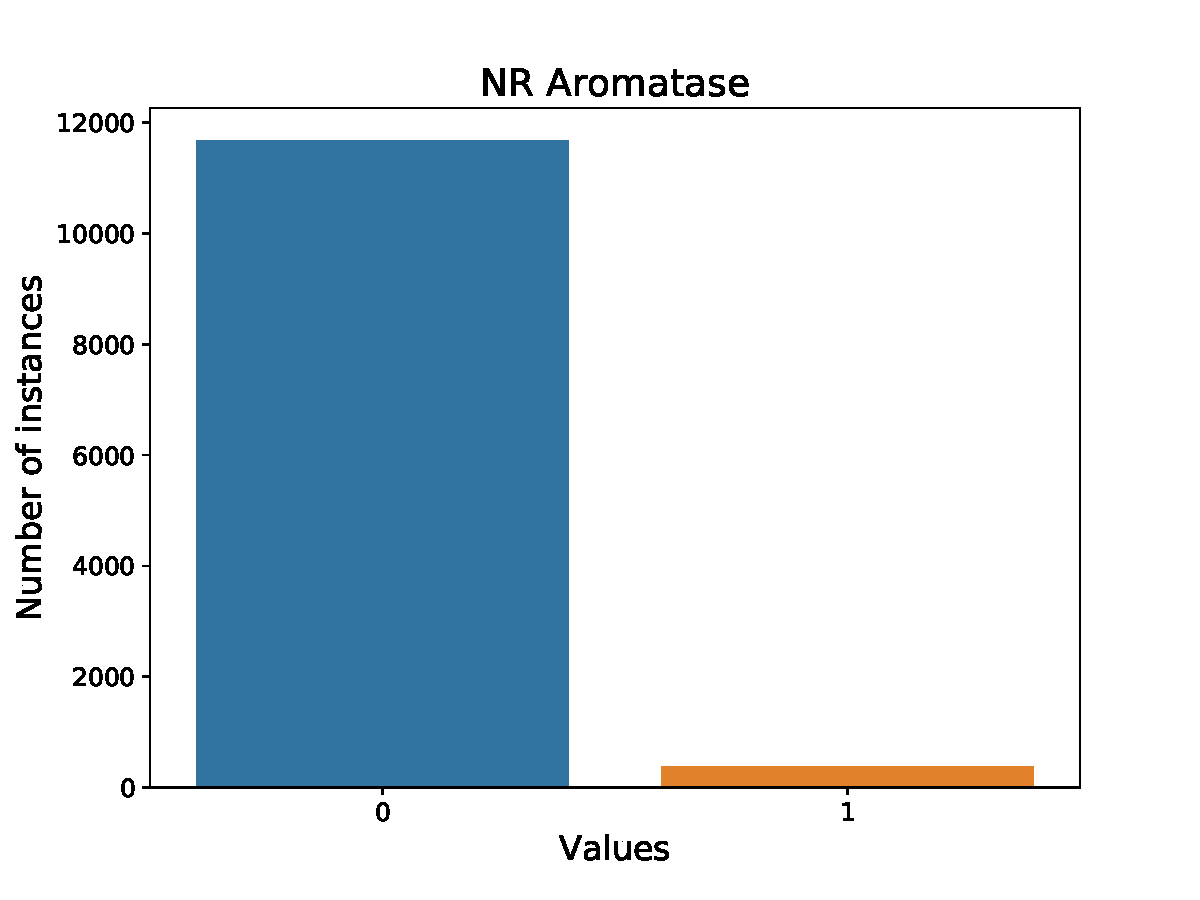
\includegraphics[width=.2\textwidth]{../images/pdf/hist-NRAromatase}}\\	\subfloat{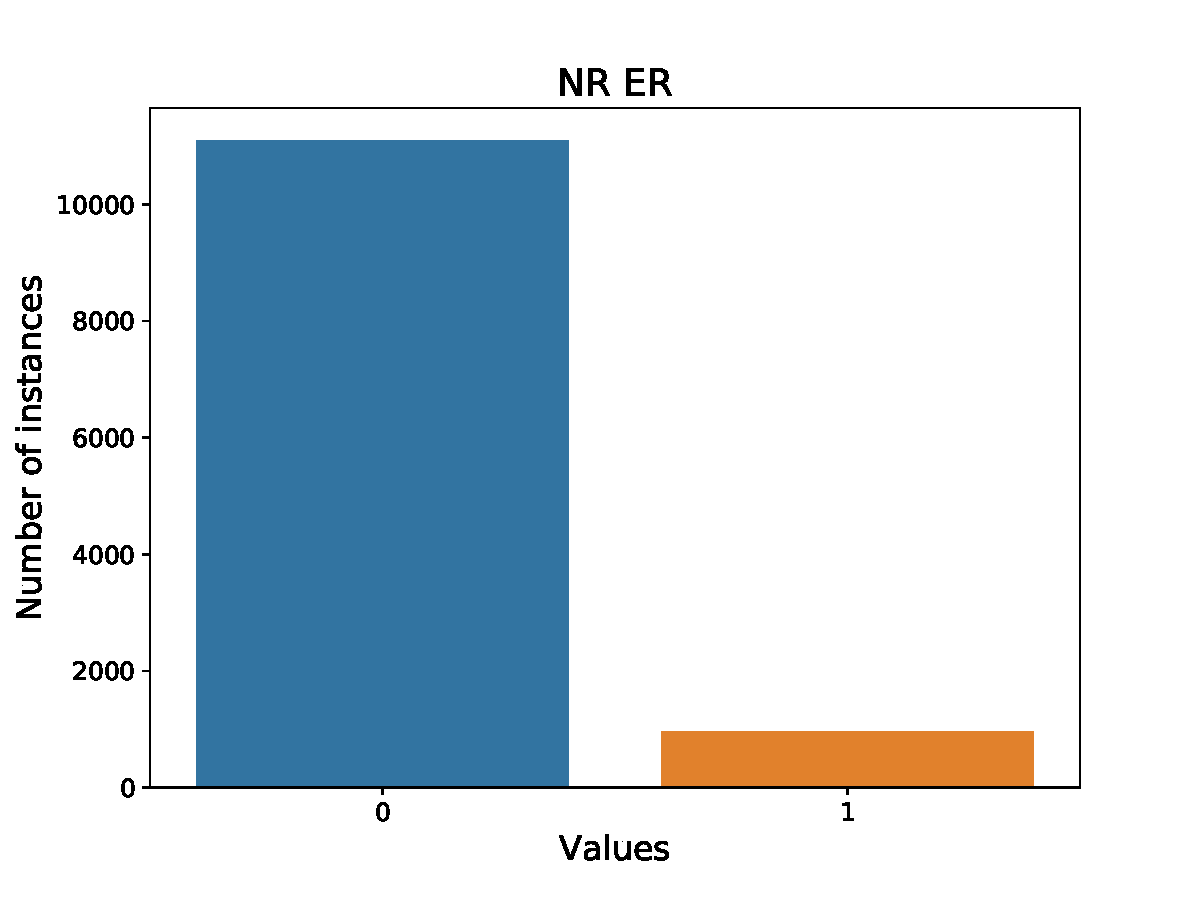
\includegraphics[width=.2\textwidth]{../images/pdf/hist-NRER}}\quad
	\subfloat{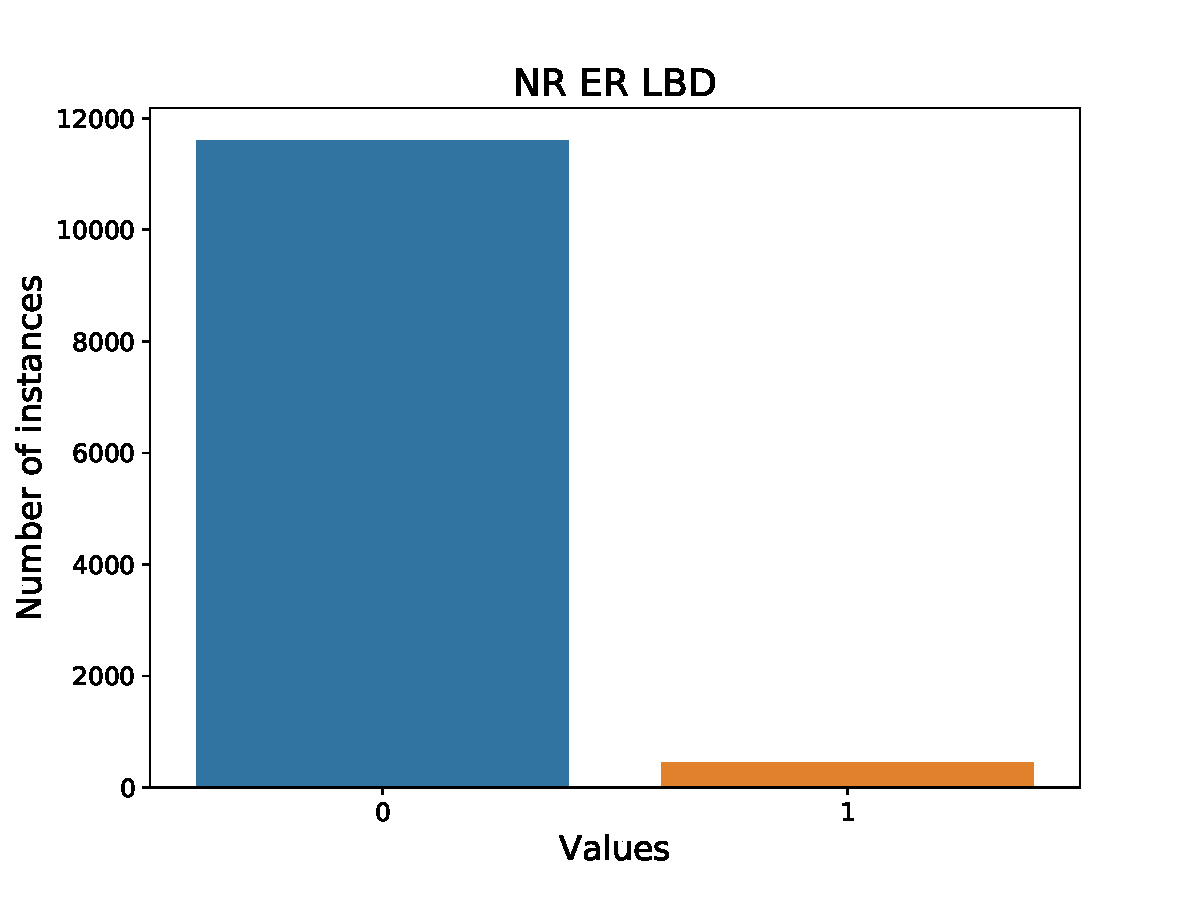
\includegraphics[width=.2\textwidth]{../images/pdf/hist-NRERLBD}}\quad
	\subfloat{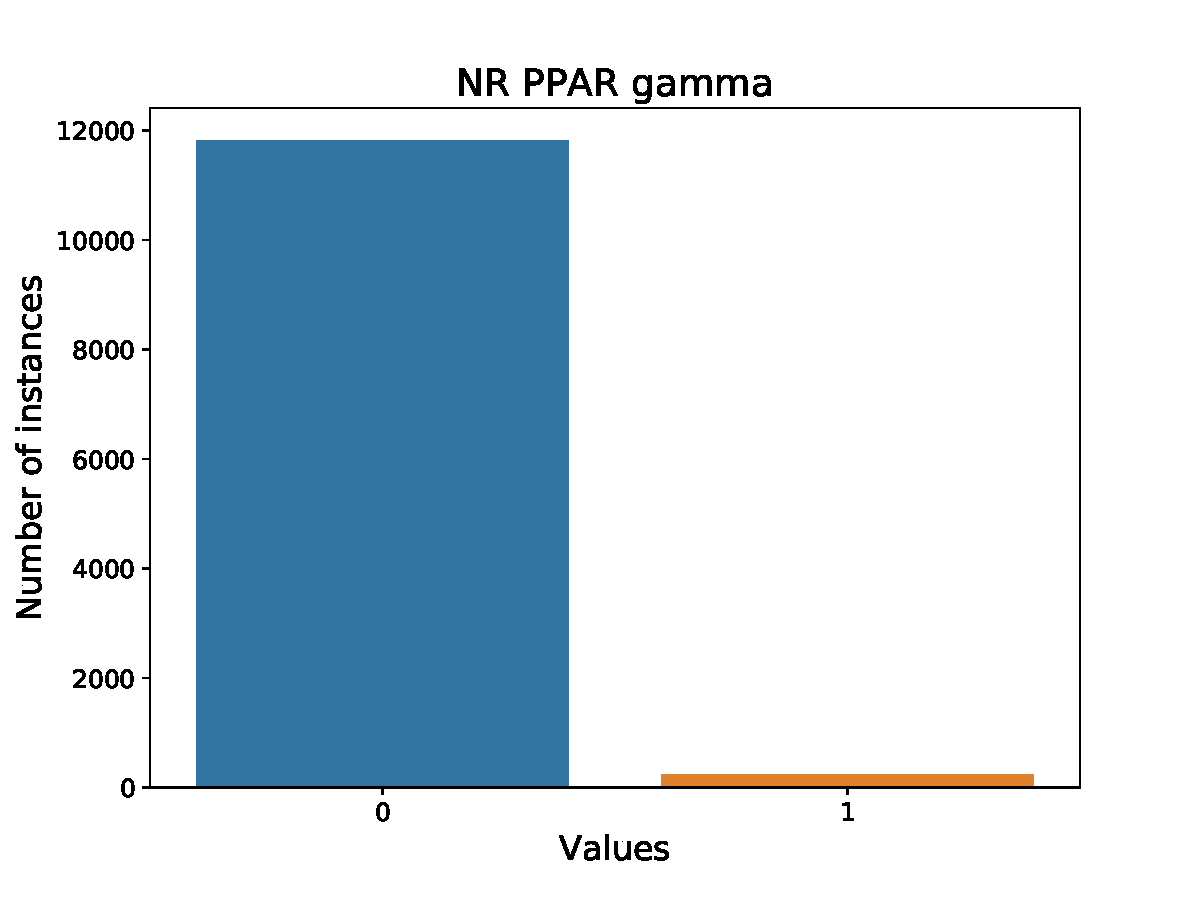
\includegraphics[width=.2\textwidth]{../images/pdf/hist-NRPPARgamma}}\quad
	\subfloat{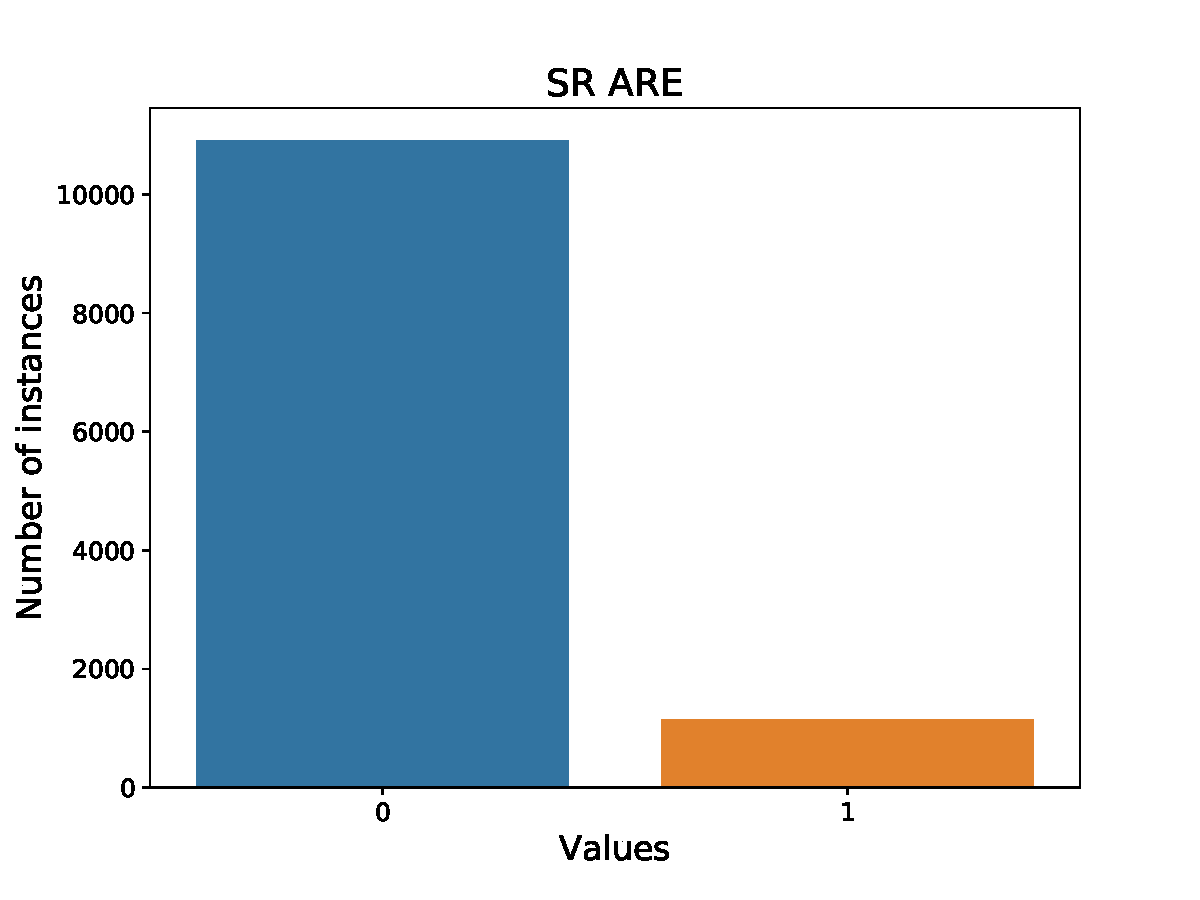
\includegraphics[width=.2\textwidth]{../images/pdf/hist-SRARE}}\\
	\subfloat{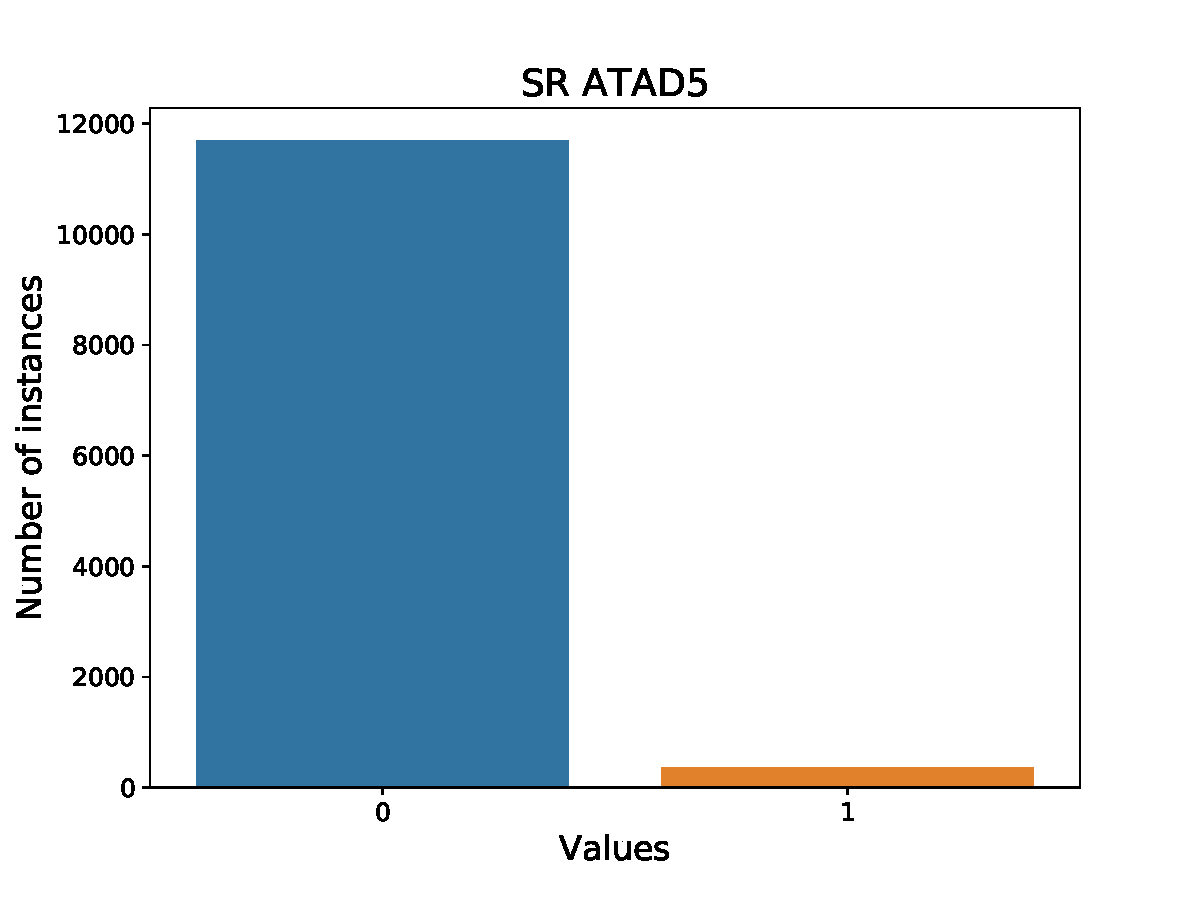
\includegraphics[width=.2\textwidth]{../images/pdf/hist-SRATAD5}}\quad
	\subfloat{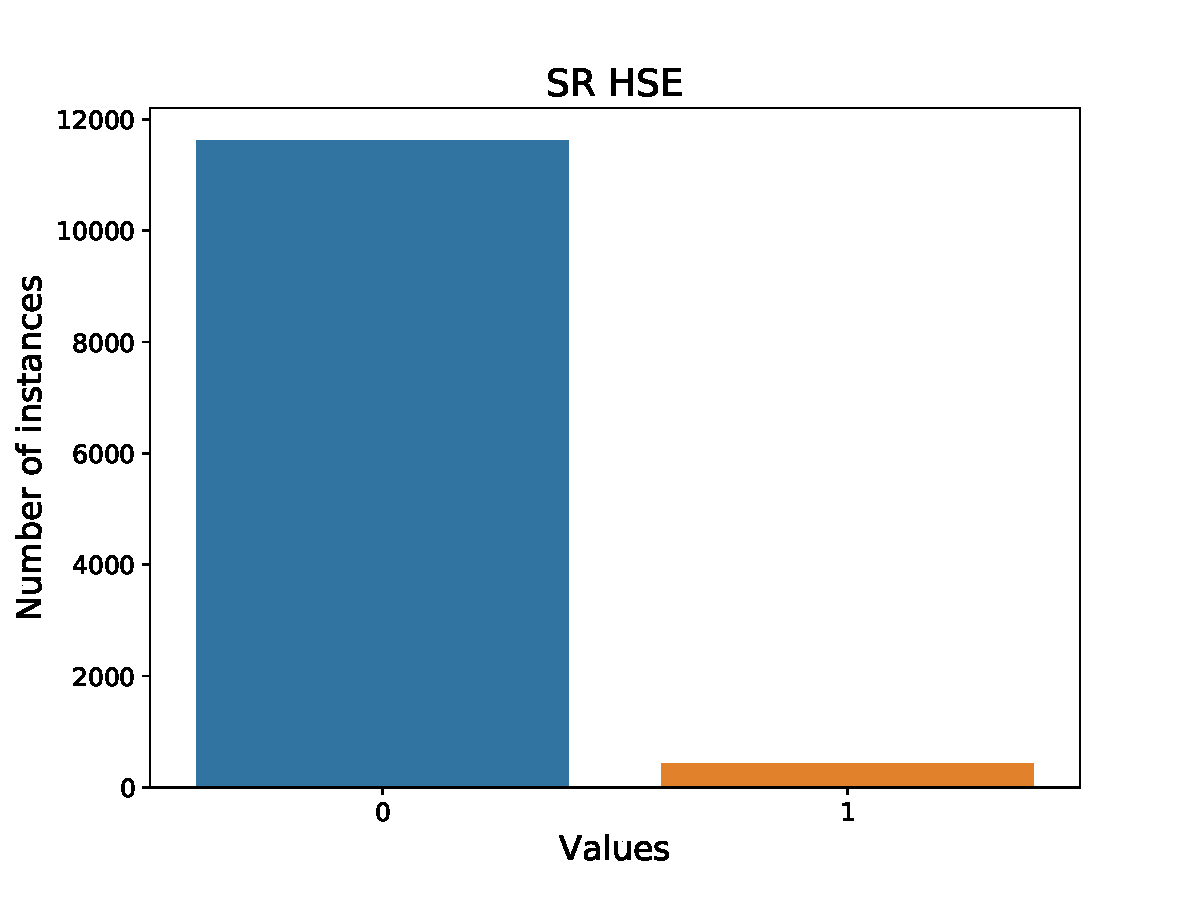
\includegraphics[width=.2\textwidth]{../images/pdf/hist-SRHSE}}\quad	\subfloat{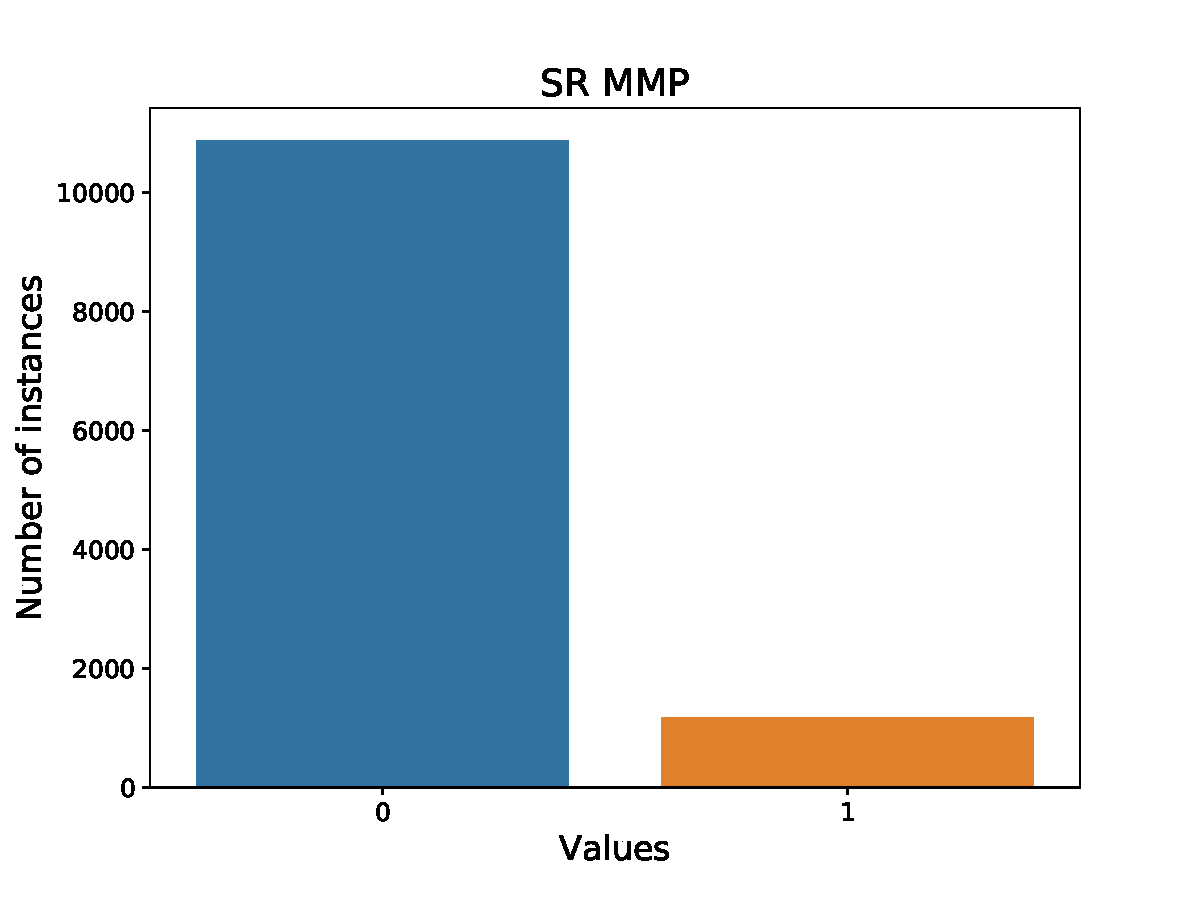
\includegraphics[width=.2\textwidth]{../images/pdf/hist-SRMMP}}\quad
	\subfloat{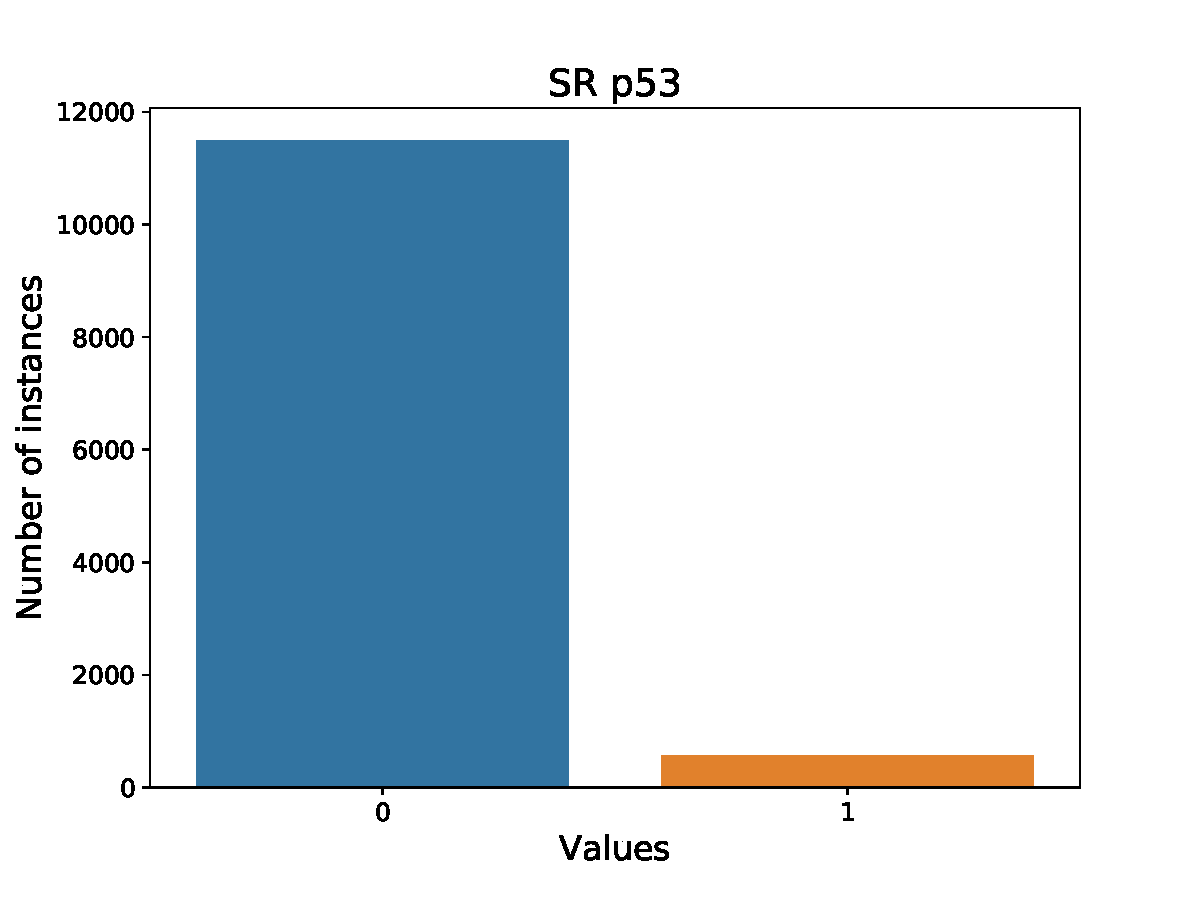
\includegraphics[width=.2\textwidth]{../images/pdf/hist-SRp53}}
	\caption{Distribuzione delle etichette dei differenti test tossicologici.}
	\label{fig:class_distribution}
\end{figure}
L'attenzione è stata poi spostata sull'analisi della distribuzione delle etichette, riportata in Figura \ref{fig:class_distribution}, che mostra un forte sbilanciamento tra il numero di 0 ed il numero di 1 per ogni classe. Come già accennato in precedenza, il problema trattato ricade sotto la categoria dei task di classificazione multi-label. Per questo motivo, anche se le classi si sono rivelate sbilanciate, non è stato possibile effettuare operazioni di \textit{over/under-sampling}, in quanto la generazione di un nuovo \textit{sample} sintetico (o la rimozione di un record nel caso complementare) per una classe avrebbe influenzato lo sbilanciamento delle classi rimanenti. \\
L'analisi della correlazione tra le etichette è stata indagata mediante una rappresentazione \textit{heatmap} della matrice di correlazione, riportata in Figura \ref{fig:labelscorrmatrixheatmap}. I valori di correlazione risultano essere molto bassi in media, salvo per due coppie di label, dove troviamo valori nell'intorno di $0.50$. Analizzando la semantica delle etichette, è emerso che le due coppie di label correlate in modo significativo riguardano l'effetto tossico in un caso sull'intero recettore, nell'altro solo su una porzione di esso.
\begin{figure}
	\centering
	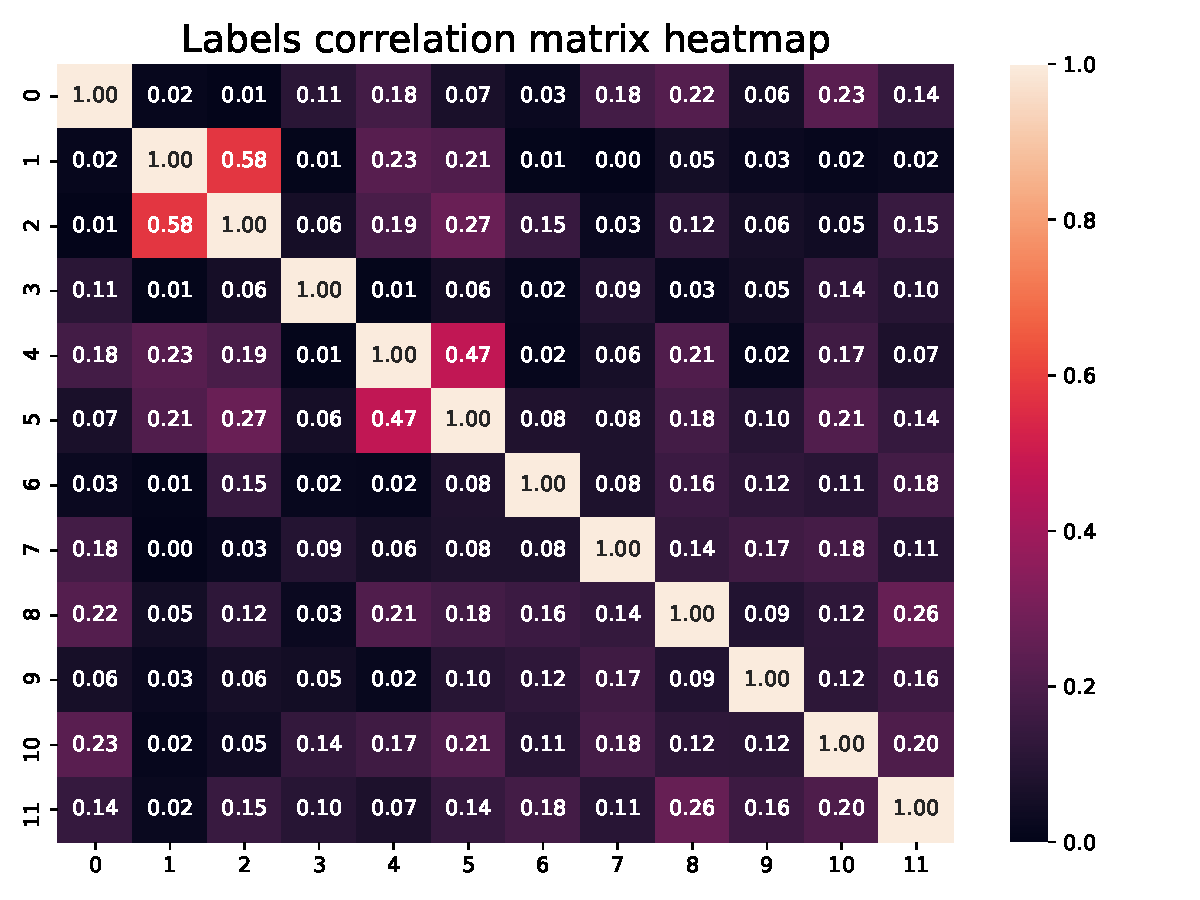
\includegraphics[width=0.7\linewidth]{../images/pdf/labels_corr_matrix_heatmap}
	\caption{Heatmap della matrice di correlazione delle feature. Solo due coppie di feature risultano correlate in modo significativo tra loro.}
	\label{fig:labelscorrmatrixheatmap}
\end{figure}

Per prima cosa è stata verificata la presenza di \textit{missing value} e il tipo dei dati contenuti nella matrice delle feature. L'analisi non ha evidenziato la presenza di alcun valore mancante e i dati si sono rivelati tutti di tipo numerico continuo. \todo{Non c'erano anche degli interi? DP Gli interi non sono forse numeri continui? MM}
Successivamente, sono state eseguite alcune operazioni di pulizia del dataset: rimuovendo $7$ feature con varianza pari a $0$ (quindi erano prive di qualsivoglia informazione) e $425$ \textit{sample} considerati come oultiler; sono stati identificati come outlier quei \textit{sample} che avessero almeno $\frac{1}{4}$ dei valori che eccedessero $3$ volte lo scarto interquantile delle relative feature.
L'analisi della correlazione tra feature e label non ha mostrato la presenza di feature altamente correlate alle label, con un valore di correlazione massimo pari a $0.35$; le feature maggiormente correlate alle diverse etichette si sono inoltre rivelate essere tutte differenti (tranne in un caso), rafforzando l'ipotesi di un'assenza di uno stretto legame tra le etichette e un'unica feature.
In Figura \ref{fig:distributionhighcorr}, è riportata un'analisi di come le varie feature/etichette sono risultate altamente correlate ($> 0.90$) con altre feature/etichette. È possibile vedere come la larga maggioranza degli elementi sia correlato con un basso numero di feature (si noti la scala logaritmica sull'asse \textit{x}).
Si trova, poi, un insieme di feature correlate con un numero di elementi compreso tra $5$ e $30$, mentre una decina di feature risultano correlate a più di 40 elementi. Questo suggerisce che sia opportuno eseguire un'operazione di feature reduction prima di eseguire l'addestramento del modello, in modo da ridurre la ridondanza di informazione e aumentando il potenziale di generalizzazione del modello; ciò permette inoltre di velocizzare sia il processo di train sia quello di inferenza. \todo[inline]{velocizzare il processo di inferenza e train mi sembra un'affermazion forte. Soprattutto per l'inferenza. Il maggior tempo di train dipende di più dai layer nascosti imho DP. Beh, meno feature significa meno dati su cui effettuare calcoli e potenzialmente una struttura più piccola della rete. Pensa solo a quando con le immagini abbassiamo la risoluzione quanto è + veloce la rete... MM}
\begin{figure}
	\centering
	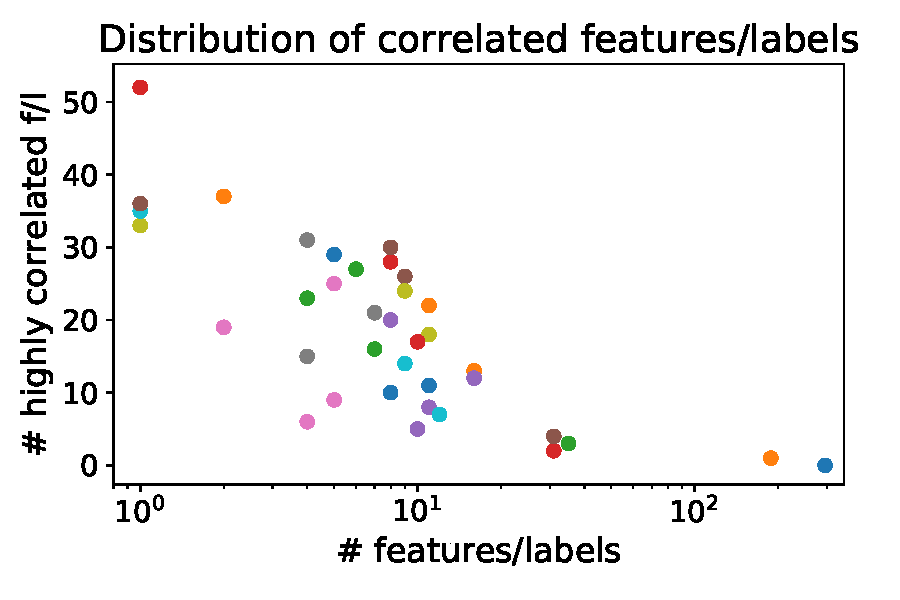
\includegraphics[width=0.7\linewidth]{../images/pdf/distribution_high_corr}
	\caption{Distribuzione di feature/label altamente correlate. È stata utilizzata la scala logaritmica per l'asse x.}
	\label{fig:distributionhighcorr}
\end{figure}
Infine, i dati sono stati  standardizzati con media nulla e deviazione standard unitaria, in modo da non creare squilibri, in termini di magnitudine dell'input dei modelli neurali presentati nelle prossime sezioni; ciò è stato fatto in quanto feature con scale differenti possono portare instabilità nella rete, causando la creazione di pesi troppo elevati che rendono le predizioni fortemente suscettibili a piccole variazioni dell'input.

\section{Approccio e metodi utilizzati}
A seguito dell'analisi sulle feature, che ha evidenziato una correlazione tra un discreto numero di esse, sono state sviluppate e utilizzate tre differenti tecniche di feature reduction. 
La prima è una feature selection basata sulla correlazione; \textit{i.e.}, elimina quegli elementi che risultano correlati oltre una certa soglia con altri elementi. 
Ponendo questa soglia a $0.90$, la dimensione dell'input passa da $793$ a $414$ feature.
Le rimanenti due tecniche utilizzate, che afferiscono ai metodi di feature extraction, sono la Principal Component Analysis (PCA) e l'utilizzo di un autoencoder; in entrambi i casi, il numero di feature estratte è stato fissato a $100$.
Per quanto concerne la struttura dell'autoencoder, è stata utilizzata una topologia con 2 layer nascosti prima del \textit{bottleneck}, i layer sono composti da un numero di neuroni dimezzato progressivamente, i quali sfruttano una \texttt{relu} come funzione di attivazione. 
Al contrario, il layer di output utilizza una funzione lineare, in quanto i valori attesi sono numeri reali.\\
Al fine di individuare la migliore topologia da utilizzare per il successivo processo di ottimizzazione sono state poste a confronto tre reti dalla profondità crescente; la struttura di base si compone di $3$ layer nascosti con attivazione \texttt{relu}, dropout $0.2$ e normalizzazione dopo l'attivazione, con rispettivamente $512$, $256$ e $128$ neuroni. 
Ad essa, sono stati aggiunti in modo incrementale due layer con le medesime caratteristiche e con numero di neuroni dimezzato rispetto al livello precedente. %(\textit{i.e.}, 64 e 32 neuroni rispettivamente). 
In coda alle reti così create è stato posto un layer di output con $12$ neuroni attivati mediante una sigmoide, poiché le label attese assumono valori pari a 0 o 1; l'ottimizzatore utilizzato per il processo di training è stato \texttt{adam} (scelto per la maggiore efficienza e il \textit{learning rate} dinamico) e il parametro di peso della funzione di \textit{loss} è stato posto a $20$ (valore prossimo allo sbilanciamento complessivo tra le classi). 
Il valore appena citato influenza il peso che la funzione di loss associa ad un errore sulla classe positiva: questa funzione di \textit{loss} permette quindi di gestire problemi fortemente sbilanciati come nel caso preso in analisi.
Il fine di questa operazione è quello di determinare se una topologia più profonda della rete sia in grado di ottenere performance migliori a parità di valori degli iperparametri.

Una volta individuata la migliore tra le topologie proposte, è stato effettuato un processo di ottimizzazione bayesiana di alcuni iperparametri del modello. 
Questa tecnica, a differenza di approcci più \textit{na\"ive}, è \textit{sample efficient}, ovvero sfrutta al meglio il budget a disposizione per individuare la configurazione ottimale degli iperparametri. 
Nel processo sono stati inclusi: (i) dimensione del \textit{batch}; (ii) valore di dropout; (iii) peso della funzione di regolarizzazione all'interno della funzione obiettivo; (iv) funzione di attivazione dei layer nascosti; (v) peso della funzione di loss per la gestione dello sbilanciamento tra le classe.
Vista la presenza di variabili sia continue che categoriche, il modello surrogato selezionato è stato quello delle \textit{random forest}, maggiormente adatto alla gestione di valori non continui. 
Il budget messo a disposizione del processo è stato fissato a 120 valutazioni, di cui il 12,5\% è stato utilizzato come \textit{initial design} del modello surrogato, mediante un campionamento dello spazio Latin Hypercube Sampling (LHS). 
Il valore ottimizzato dal processo è stato il valore medio delle AUC (Area Under Curve) sulle $12$ classi in \textit{3-fold cross validation}; la funzione di acquisizione utilizzata è stata la Lower Confidence Bound (LCB).
Il processo di Automated Machine Learning (AutoML) è stato effettuato considerando separatamente come input della rete sia il dataset ottenuto dopo la fase di \textit{preprocessing}, sia le tre tecniche di feature reduction (applicate al dataset dopo le operazioni di pulizia).
Così facendo, è stato possibile individuare la configurazione di iperparametri ottimi per i vari possibili input e confrontare le performance dei modelli associati ad essi.

Avendo stabilito la combinazione tra feature reduction e iperparametri in grado di massimizzare la AUC media, è stato quindi analizzato il modello derivante più nel dettaglio.
Il classificatore così ottenuto è stato utilizzato come metodo di predizione per i dati di test e le performance ottenute sono state confrontate con quelle dei modelli proposti in letteratura.
Oltre a considerare le AUC inerenti alle singole classi e media, sono state analizzate le curve Receiver Operating Characteristic (ROC) riguardanti le singole classi e si è studiato come all'evolvere della percentuale di True Positive (\%TP) desiderata, evolvono le misure di precision e recall inerenti alle singole classi.

\section{Risultati ottenuti}
The Results section is dedicated to presenting the actual results (i.e. measured and calculated quantities), not to discussing their meaning or interpretation. The results should be summarized using appropriate Tables and Figures (graphs or schematics). Every Figure and Table should have a legend that describes concisely what is contained or shown. Figure legends go below the figure, table legends above the table. Throughout the report, but especially in this section, pay attention to reporting numbers with an appropriate number of significant figures. 

\todo[inline]{risultati reti profonde diverse in tabella DP}

Invece, per quanto concerne il processo di ottimizzazione degli iperparametri, i valori di \textit{best seen} per ogni possibile input della rete (una delle tecniche precedenemente descritte di feature reduction o l'utilizzo di nessuna di esse) sono riportati in Tabella \ref{tab:bestseen}. 
Inoltre, in Figura \ref{fig:best-seen} è riportata l'evoluzione del valore di \textit{best seen} ad ogni \textit{step} del processo di ottimizzazione per tutte le possibili strategie di input della rete.
In aggiunta, in Figura \ref{fig:auc-iteration} è riportato il valore di AUC media ottenuto con l'\textit{i}-esima configurazione durante il processo di ottimizzazione.

\begin{table}
	\centering
	\caption{Tabella riportante per ogni tecnica di feature reduction il valore di AUC media sulle 12 label della configurazione ottima di iperparametri, individuata da un processo di ottimizzazione SMBO.}
	\begin{tabular}{c|c}
		\label{tab:bestseen}
		\textbf{Tecnica utilizzata} & \textbf{AUC media} \\
		Nessuna & 0.837 \\ 
		Correlazione & 0.836 \\ 
		PCA & 0.822 \\ 
		Encoder & 0.821 \\ 
	\end{tabular}
\end{table}

\begin{figure}
	\begin{tabular}{cc}
		\subfloat[\label{subfig:best-seen}Sull'asse delle \textit{x} è riportata l'iterazione del processo di ottimizzazione, mentre sull'asse delle \textit{y} il valore di AUC media ottenuto dalla configurazione considerata \textit{best seen} fino a quel momento.]{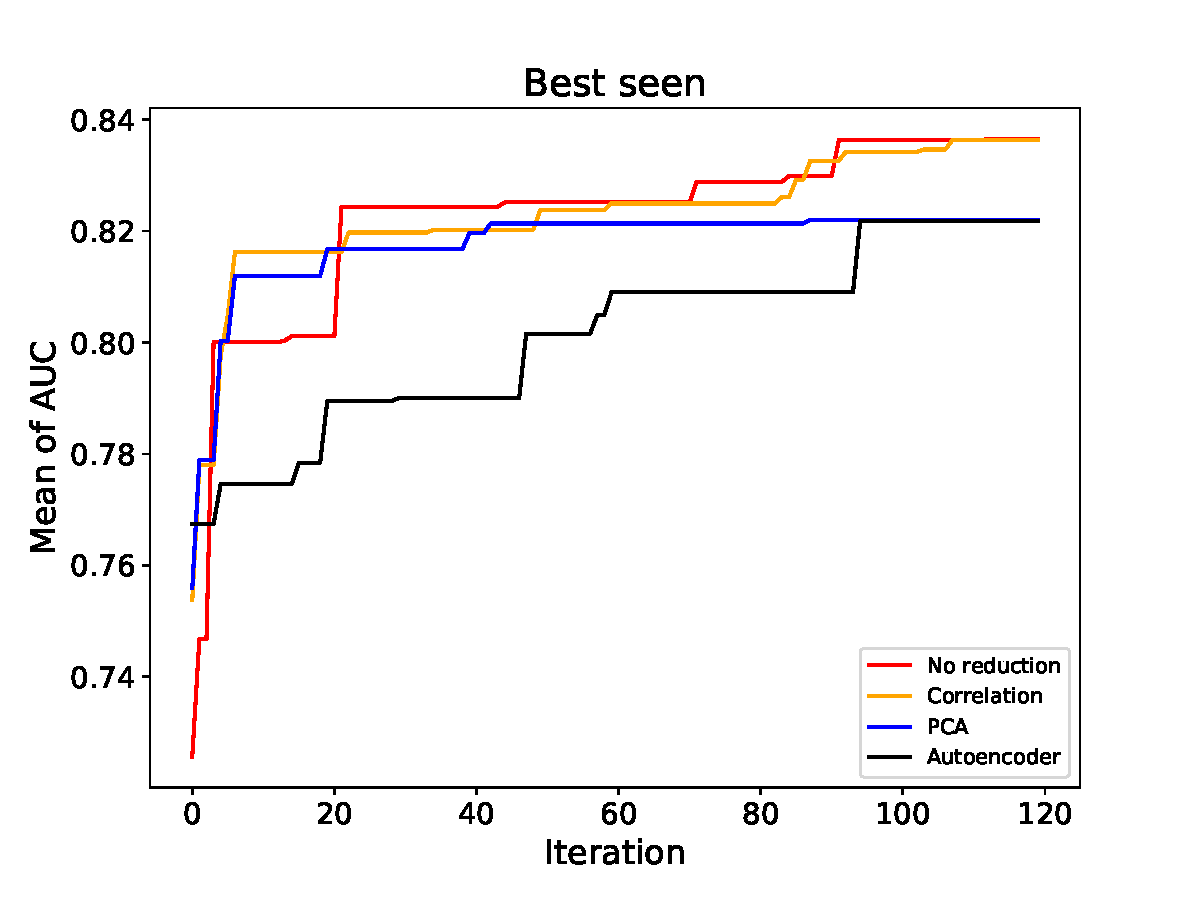
\includegraphics[width = .5\textwidth]{../images/pdf/best-seen}} &
		\subfloat[\label{subfig:auc-iteration}Sull'asse delle \textit{x} si riporta l'\textit{i}-esima iterazione del processo di ottimizzazione, sull'asse delle \textit{y} si riporta il relativo valore di AUC media ottenuto in quello \textit{step}.]{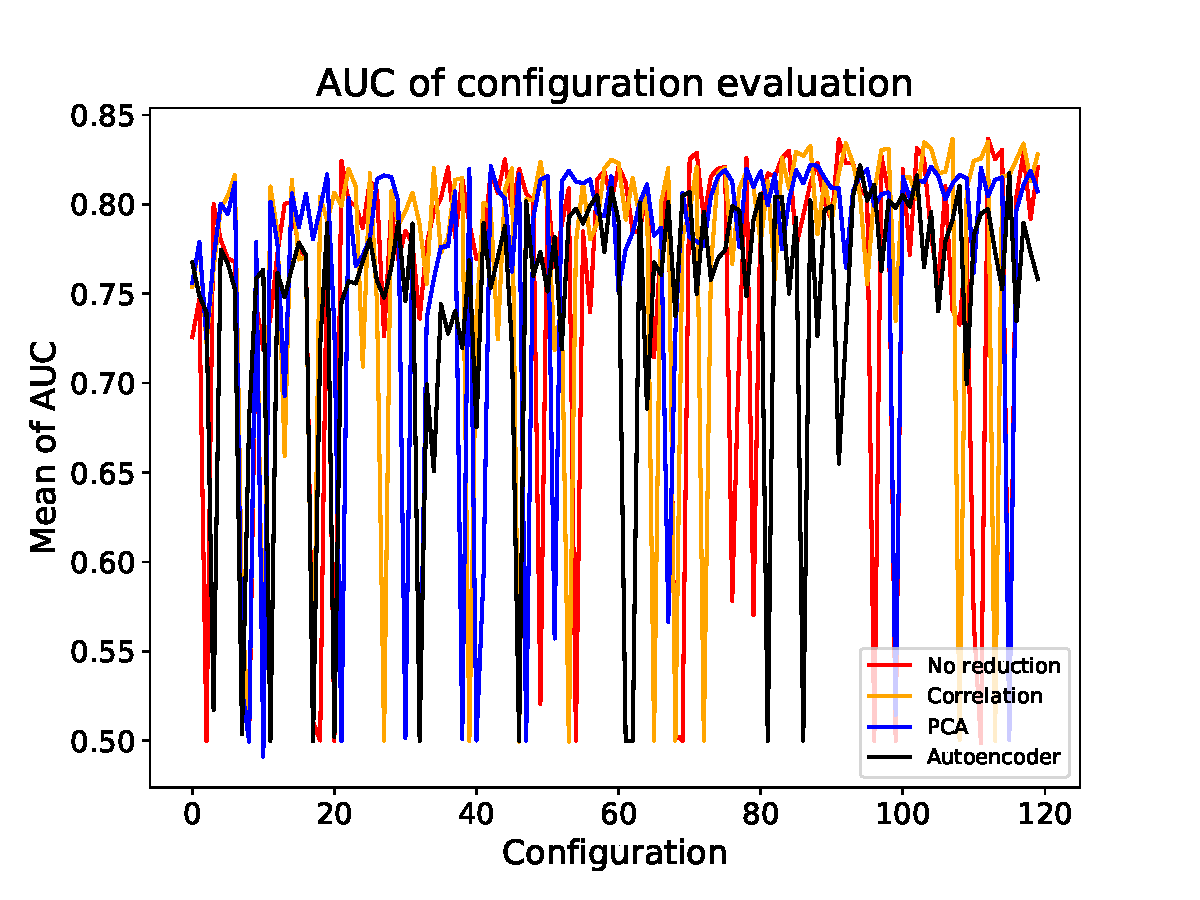
\includegraphics[width = .5\textwidth]{../images/pdf/AUC-iteration}} 
	\end{tabular}
	\caption{In Figura \ref{subfig:best-seen} è riportata l'evoluzione del \textit{best seen} durante il processo di ottimizzazione, mentre in Figura \ref{subfig:auc-iteration} ivalore di AUC media all'\textit{i}-esima iterazione.}
	\label{fig:HPO}
\end{figure} 

Infine, si riportano i risultati riguardanti le analisi sul modello considerato ottimale, ovvero quello con la strategia scelta di feature reduction e i relativi iperparametri ottimi. 
In Figura \ref{subfig:roc} si riportano le ROC \todo{mettere significato se non le si nomina prima} per ogni label, mentre in Figura \ref{subfig:pr} si riporta come all'evolvere della percentuale di \textit{True Positive} (\%TP) desiderata, evolvono la recall e precision del modello, calcolate in media sulle dodici label (linea continua), mentre l'area colorata rappresenta la deviazione standard.
Per concludere, in Figura \ref{fig:comparison} sono rappresentate le performance del modello proposto in questo lavoro e degli altri elencati nel lavoro di riferimento \cite{mayr2016deeptox}, sono confrontati per valore di AUC per ognuna delle 12 label, per media delle AUC su tutte le label (AVG), media delle AUC delle label inerenti ai \textit{stress responde effects} (SR) e delle \textit{nuclear receptor effects} (NR) \todo{citare direttamente NR e SR se già prima diciamo per cosa stanno. DP}.

\begin{figure}
	\begin{tabular}{cc}
		\subfloat[\label{subfig:roc}ROC rispettive alle dodici label, sono state calcolate usando il modello con la strategia di feature reduction scelta e relativa configurazione di iperparametri ottimi.]{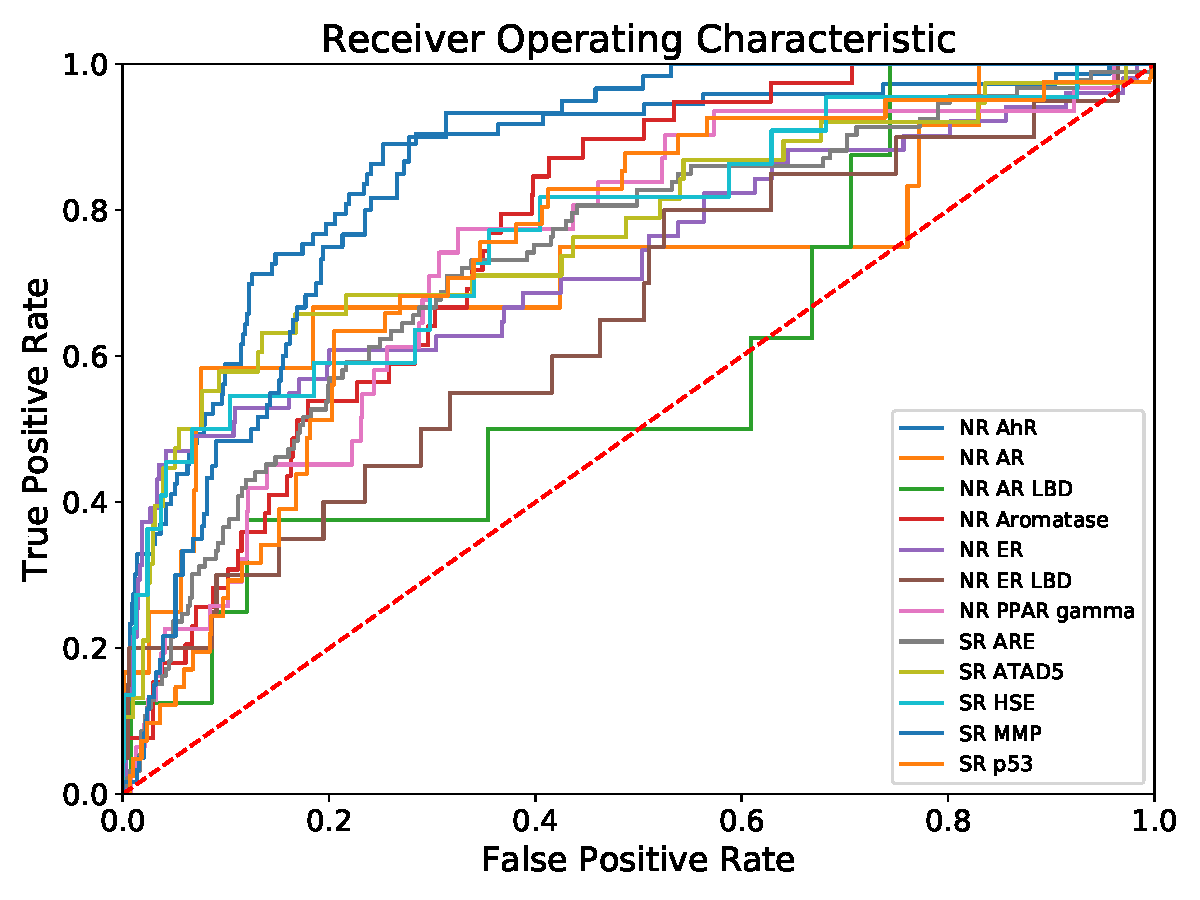
\includegraphics[width = .5\textwidth]{../images/pdf/ROC}} &
		\subfloat[\label{subfig:pr}Raffigurazione di come all'evolvere del \%TP variano i valori di precision e recall del modello.]{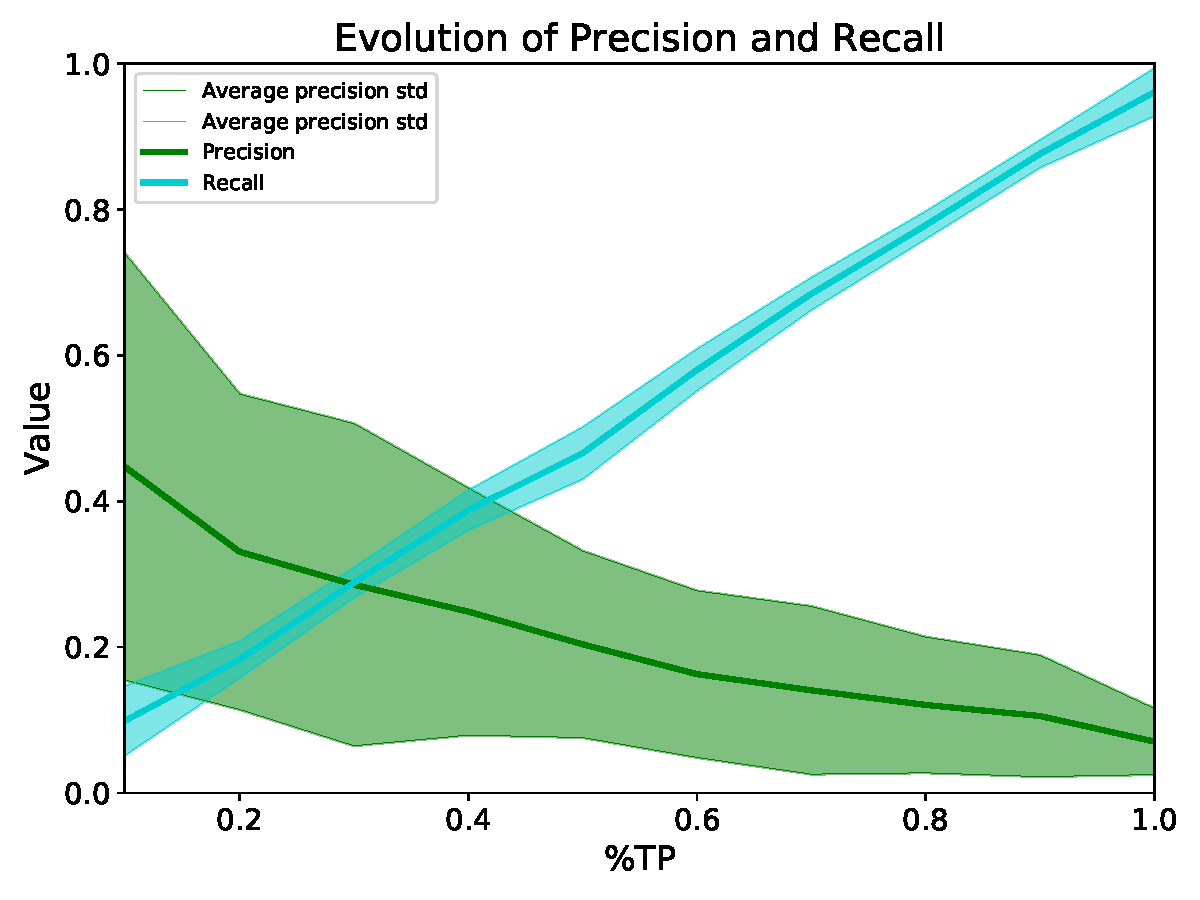
\includegraphics[width = .5\textwidth]{../images/pdf/pr_evolution}} 
	\end{tabular}
	\caption{In Figura \ref{subfig:roc} si mostrano le ROC relative alle 12 label, mentre in Figura \ref{subfig:pr} l'evoluzione di precision e recall all'aumentare del \%TP richiesto.}
	\label{fig:roc-pr}
\end{figure} 

\begin{figure}
	\centering
	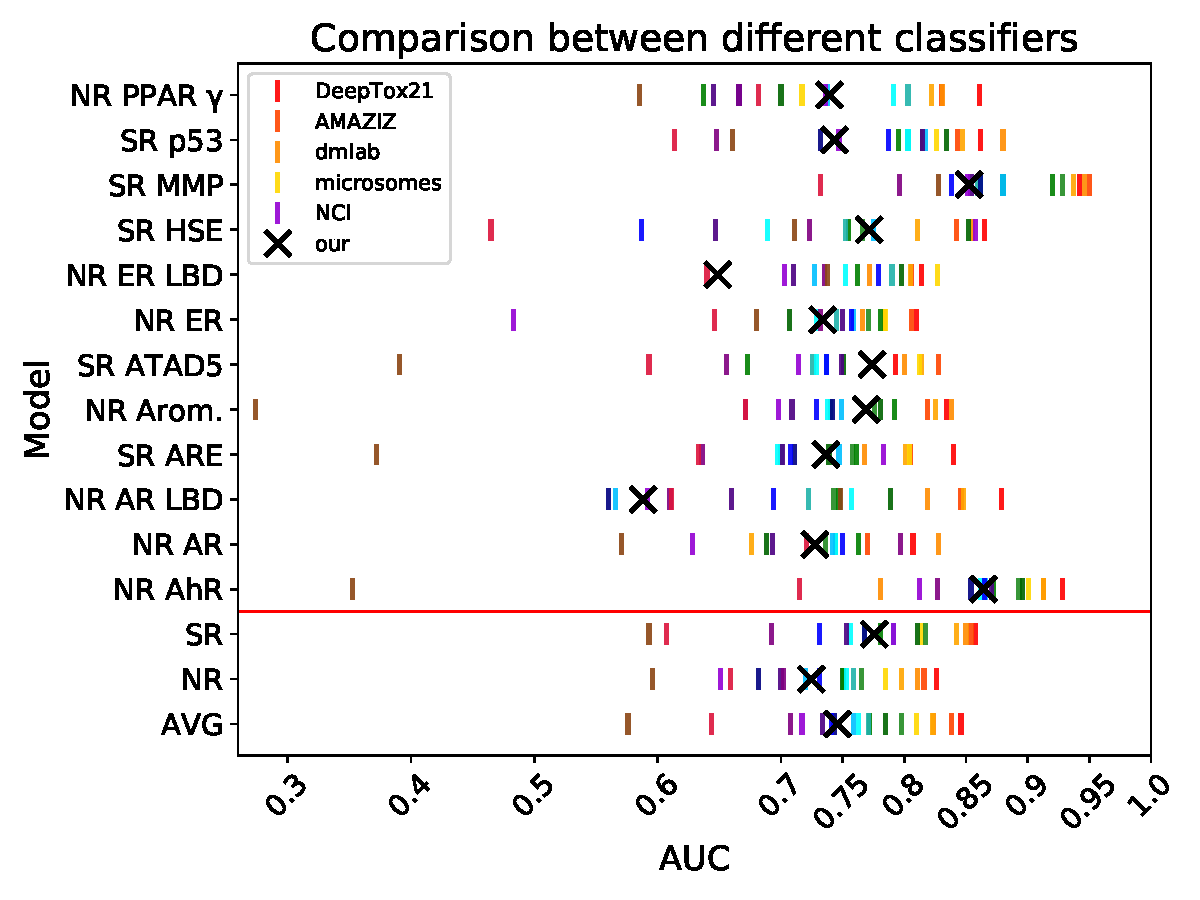
\includegraphics[width=0.9\linewidth]{../images/pdf/comparison}
	\caption{Confronto di vari modelli rispetto alle AUC (o media di AUC). Le linee rappresentano i modelli elencati nel lavoro di riferimento \cite{mayr2016deeptox}, mentre con la 'X' si indica il modello presentato in questo lavoro. Oltre alle AUC rispettive delle 12 label, sotto la linea rossa sono presentati i valori medi su tutte le label (AVG), solo sulle label relative agli SR e alle NR. Sono riportati in legenda (oltre al modello di questo lavoro) i modelli che sono risultati tra i primi due per quanto riguarda una label o una delle medie.}
	\label{fig:comparison}
\end{figure}


\todo[inline]{il grafico del learning process non lo metterei qui ma quando discutiamo se ci serve. qui lo ritengo inutile DP}

\section{Analisi dei risultati}
Le performance prodotte dalle differenti topologie di reti, riportate in Tabella \ref{tab:topology}, non mostrano differenze sostanziali; per questo motivo, seguendo il principio del rasoio di Occam, è stata selezionata la topologia più semplice, ovvero una rete a tre layer nascosti con rispettivamente $512$, $256$ e $128$ neuroni. Il risultato ottenuto mostra che non è necessario un elevato livello di profondità della rete per risolvere il problema, e che aumentare il numero di layer non apporta benefici alla performance analizzata.\\

Fissata questa topologia, il processo di ottimizzazione degli iperparametri è stato iterato per le varie tecniche di \textit{feature reduction} disponibili, oltre al dataset dopo la fase di \textit{data cleaning}. I risultati, riportati in Figura \ref{fig:HPO}, mostrano l'andamento del processo di ricerca degli iperparametri ottimi. In Figura \ref{subfig:best-seen} è possibile apprezzare come la tecnica di eliminazione delle feature correlate, unita al non utilizzo di alcuna \textit{feature reduction}, riescano a garantire performance leggermente migliori rispetto a tecniche di \textit{feature extraction} quali PCA e autoencoder, che trovano configurazioni collegate a valori di AUC identici nel grafico. Considerando il fatto che i due approcci appena nominati portano ad una drastica riduzione del numero di input della rete (da $\sim800$ a $100$ elementi), possiamo dedurre che entrambi gli approcci riescano a mantenere la quasi totalità dell'informazione utile contenuta nelle feature di partenza. In Figura \ref{subfig:auc-iteration} è invece riportata l'AUC associata alle varie iterazioni dell'ottimizzazione per i quattro test effettuati. Dal grafico emerge come il processo, per ogni input proposto, analizzi principalmente lo spazio nell'intorno dei valori ottimi già individuati, salvo esplorare sporadicamente configurazioni associate a performance notevolmente peggiori (depressioni nella curva associata al metodo).\\
Considerata la differenza di performance mostrata dalle differenti tecniche di \textit{feature reduction} e la limitatà complessità di addestramento delle rete, è stato deciso di utilizzare la correlazione come metodo di riduzione della dimensionalità dell'input. Questa, nel nostro caso, permette di dimezzare il numero di feature in input, garantendo comunque un valore di AUC ottimale, come riportato dal processo di ottimizzazione. Un approccio più drastico in termini di riduzione della dimensionalità, come PCA e autoencoder con numero di feature limitate a $100$, avrebbe senso nel caso in cui l'addestramento della rete richiedesse molte più risorse computazionali: in questo caso, il \textit{tradeoff} tra la perdita di performance e il guadagno in termini di tempo di addestramento e inferenza della rete avrebbe sicuramente senso.\\

Avendo selezionato la topologia, la tecnica di riduzione della dimensionalità e gli iperparametri ottimali per il nostro problema, il modello derivante è stato addestrato sull'intero dataset e le performance finali sono state valutate mediante il testset.
In Figura \ref{subfig:roc} sono riportate le curve ROC relative alle varie etichette del dataset; queste curve, oltre ad essere utilizzate per calcolare l'AUC utilizzata come misura di performance del problema, permettono di selezionare i \textit{threshold} di predizione associati alle varie classi. Modificando questi valori, è possivile ottenere una percentuale di Veri Positivi a piacere, a discapito ovviamente della percentuale di Falsi Positivi. Allo stesso modo, fissando una percentuale di Veri Positivi maggiore, il valore della \textit{Recall} per classe cresce, a discapito della \textit{Precision}, come mostrato in Figura \ref{subfig:pr}. A questo punto, visto il dominio di applicazione del problema, sarebbe necessaria una conoscenza esterna del reale costo associato ai valori della matrice di confusione delle varie classi al fine di selezionare i differenti \textit{threshold} (e quindi le percentuali di Veri Positivi): possiamo supporre che un Falso Positivo abbia un costo sensibilmente inferiori rispetto ad un Falso Negativo, in quanto una molecola tossica non rilevata appare essere un rischio ben più grave rispetto ad una molecola innocua classificata come dannosa.\\

L'approccio realizzato è stato poi confrontato con i metodi presenti nello stato dell'arte, producendo il grafico in Figura \ref{fig:comparison}. È possibile affermare che la tecnica proposta si posiziona circa a metà classifica come performance medie, con posizionamenti variegati a seconda delle classi. Si evidenzia come l'approccio proposto consente l'inferenza di tutte e dodici le classi e non è un metodo \textit{ensamble}, a differenza della maggioranza degli approcci presenti nel grafico.



\section{Conclusioni}
Conclusions should summarize the central points made in the Discussion section, reinforcing for the reader the value and implications of the work. If the results were not definitive, specific future work that may be needed can be (briefly) described. The conclusions should never contain ``surprises''. Therefore, any conclusions should be based on observations and data already discussed. It is considered extremely bad form to introduce new data in the conclusions.



\bibliographystyle{IEEEtran}
\bibliography{references.bib}

\end{document}